




\begin{figure*}[!htb]

\minipage{0.31\textwidth}%
  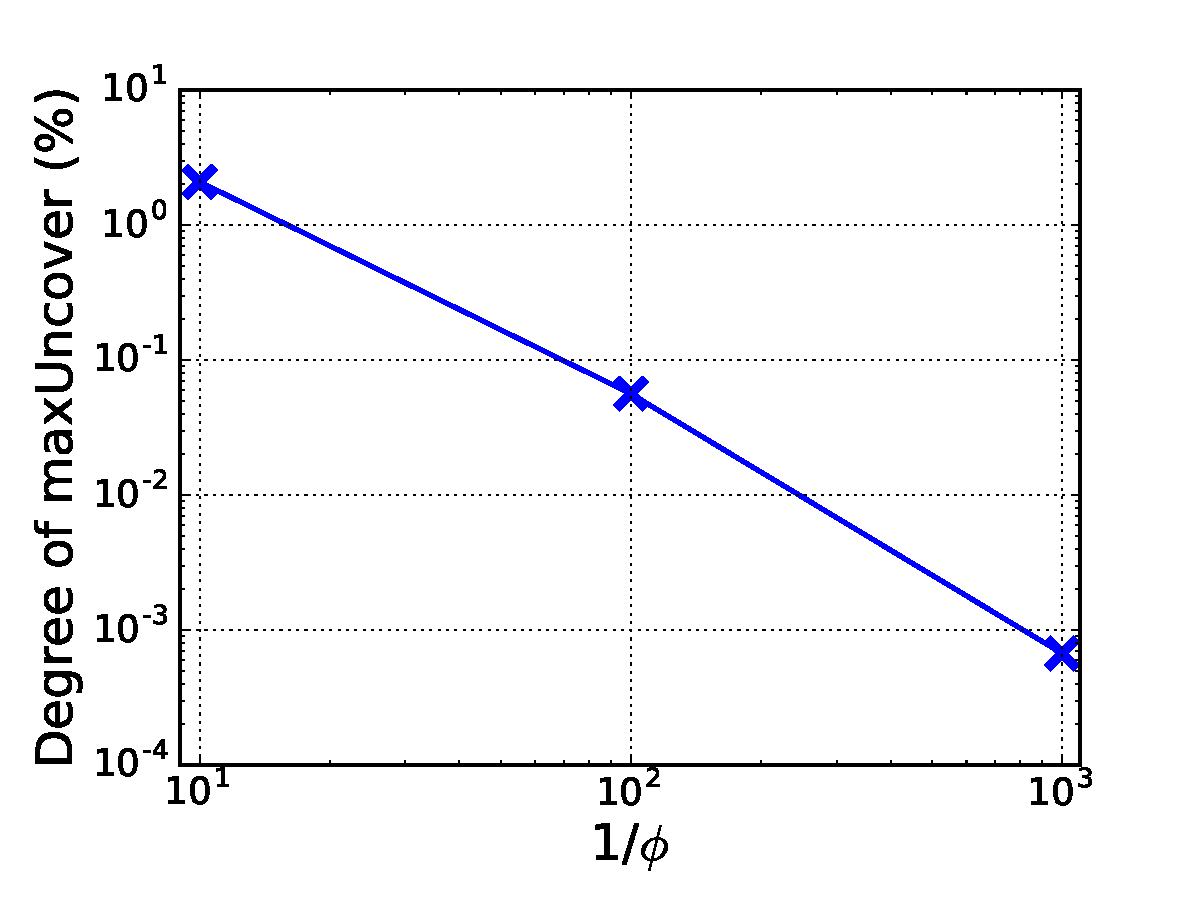
\includegraphics[width=\linewidth]{figure/maxUncover.pdf}
  \mycaption{fig:maxUncover}{Relation between $\phi$ and degree of maxUncover.}
  {
  How the degree of maxUncover changes with the change of $\phi$ from $10^{-1}$ to $10^{-3}$.
  }
  %\label{fig:aveUncover}
\endminipage\hfill
\minipage{0.31\textwidth}%
  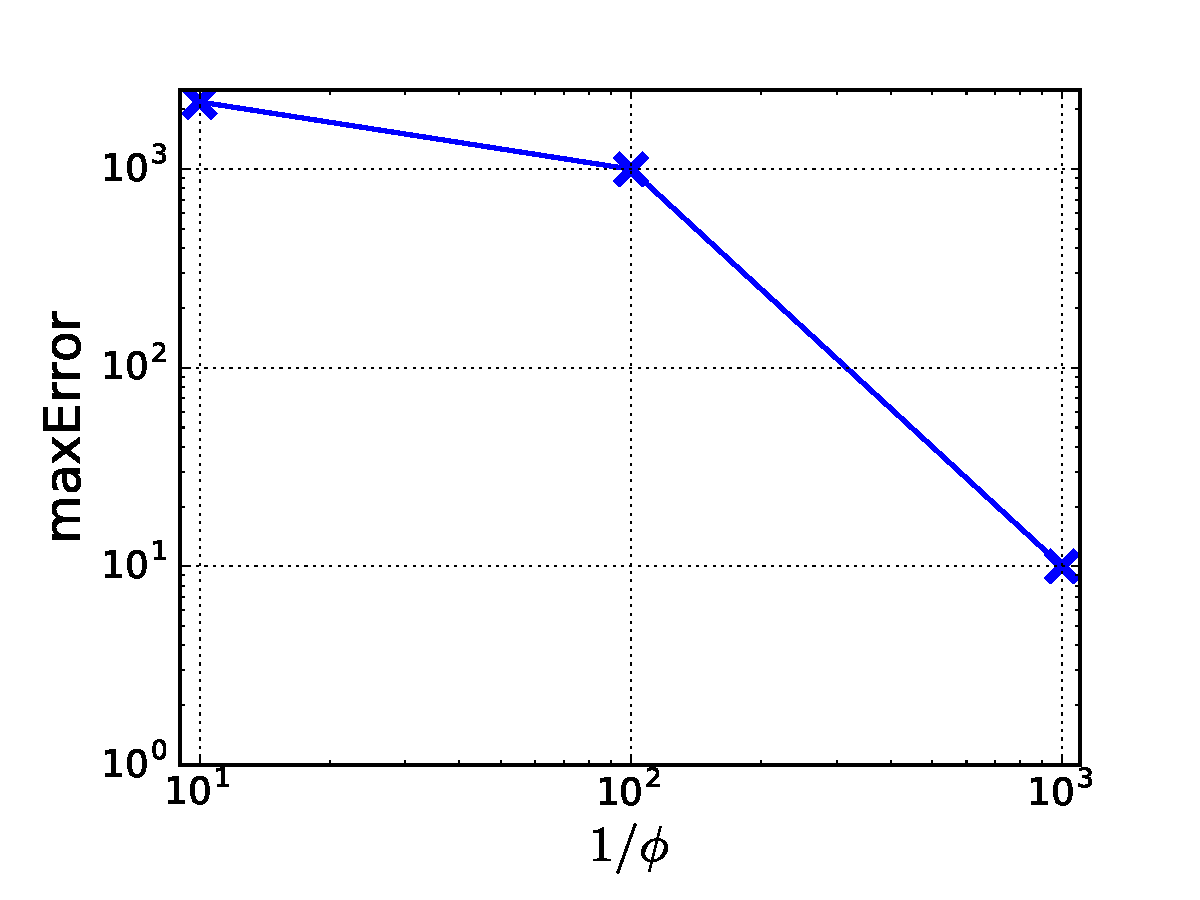
\includegraphics[width=\linewidth]{figure/maxError.pdf}
  \mycaption{fig:maxError}{Relation between $\phi$ and maxError.}
  {How maxError changes with the change of $\phi$ from $10^{-1}$ to $10^{-3}$.}
  %\caption{Relation between $\phi$ and maxError.}
  %\label{fig:maxError}

\endminipage\hfill
\minipage{0.31\textwidth}%
  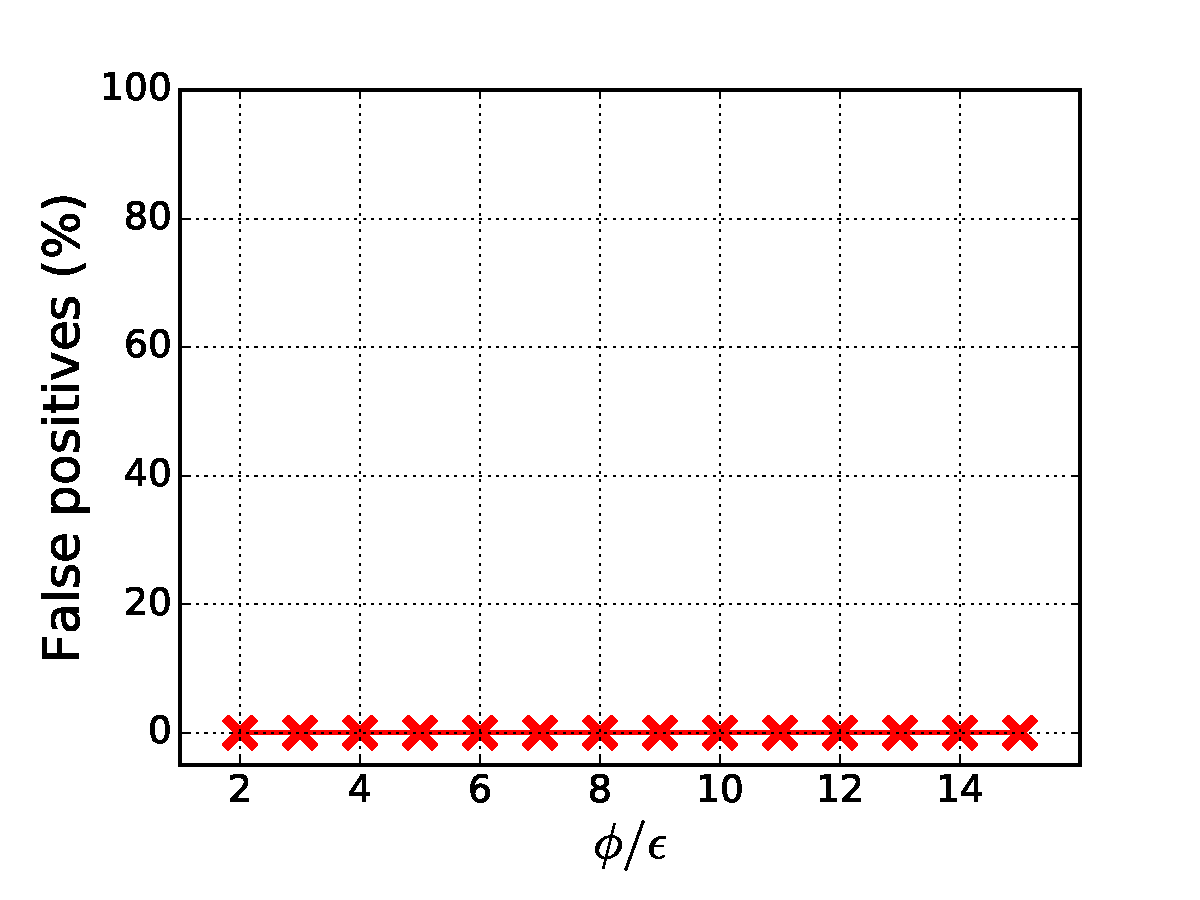
\includegraphics[width=\linewidth]{figure/fp}
  \mycaption{fig:fp}{False positives.}
{False positives in $(\phi, \epsilon)\mbox{-}HMF$ as a function of $\epsilon$. The value of $\phi$ is fixed to $10^{-2}$.
The value of $\phi/\epsilon$ changes from 2 to 15.}
  
\endminipage
\vspace{-0.1in}
\end{figure*}